
\chapter{Fitting the Spectra}

Fitting of the spectra involves selecting a spectral line of interest (e.g. \ion{Fe}{12} 195.12\,\AA) from the spectral windows of the data and determining a guess on the fit parameters. The next ingredient for a fit is the selection of an optimization method\sidenote{Here we use a Python implementation of the well-known IDL method mpfit which solves the non-linear least squares problem using the Levenberg-Marquardt algorithm. The Python implementation mpfit.py is found on GitHub (https://github.com/segasai/astrolibpy/) and included in our analysis software.}.

For this we've created a set of fit templates for different spectral lines. An \verb+h5dump+ on the file shows that it contains a \verb+/template+ group for the initial guess on the fit parameters and a \verb+/parinfo+ group containing constraints on the parameters for \verb+mpfit.py+.

\begin{lstlisting}
h5dump -n fe_12_195_119.2c.template.h5
HDF5 "fe_12_195_119.2c.template.h5" {
FILE_CONTENTS {
 group      /
 group      /parinfo
 dataset    /parinfo/fixed
 dataset    /parinfo/limited
 dataset    /parinfo/limits
 dataset    /parinfo/tied
 dataset    /parinfo/value
 group      /template
 dataset    /template/component
 dataset    /template/data_e
 dataset    /template/data_x
 dataset    /template/data_y
 dataset    /template/fit
 dataset    /template/fit_back
 dataset    /template/fit_gauss
 dataset    /template/line_ids
 dataset    /template/n_gauss
 dataset    /template/n_poly
 dataset    /template/order
 dataset    /template/wmax
 dataset    /template/wmin
 }
\end{lstlisting}

 The object \verb+eis_read_template.py+ can be used to read a template file and examine the contents.

\begin{lstlisting}
from eis_read_template import eis_read_template
filename = 'fe_12_195_119.2c.template.h5'
template = eis_read_template(filename)
\end{lstlisting}

This produces the output below, showing the \verb+/parinfo+ group that contains  parameters (peak, centroid, width, background) for a double Gaussian fit along with the parameter constraints. Note that this is specific to using the \verb+mpfit+ method (see the GitHub page for more info).
\begin{lstlisting}
+ template file = fe_12_195_119.2c.template.h5
*PARAMETER CONSTRAINTS*
*              Value      Fixed            Limited                 Limits               Tied
 p[0]     57514.6647          0          1          0       0.0000       0.0000
 p[1]       195.1179          0          1          1     195.0778     195.1581
 p[2]         0.0289          0          1          1       0.0191       0.0510
 p[3]      8013.4013          0          1          0       0.0000       0.0000
 p[4]       195.1779          0          1          1     195.1378     195.2181          p[1]+0.06
 p[5]         0.0289          0          1          1       0.0191       0.0510          p[2]
 p[6]       664.3349          0          0          0       0.0000       0.0000
 \end{lstlisting}

 Next you'll want to prep the data for fitting. Once you've read in a template file, you can use the central wavelength to find the desired spectral window in the data using \verb+eis_read_raster+ as shown in the previous chapter.

\begin{lstlisting}
from eis_read_raster import eis_read_raster
from eis_read_template import eis_read_template

# input data and template files
file_data     = 'eis_20190404_131513.data.h5'
file_template = 'fe_12_195_119.2c.template.h5'

# read fit template
template = eis_read_template(file_template)

# get central wavelength
wmin = template.template['wmin']
wmax = template.template['wmax']
wave = wmin + (wmax-wmin)*0.5

# read raster
raster = eis_read_raster(file_data, wave)
ints   = raster.data['data']
wave   = raster.data['wave']
corr   = raster.data['wave_corr']
\end{lstlisting}

Prepping of the data can be handled at various levels of sophistication at the user's discretion, however, at a minimum it should include handling bad values\sidenote{Negative values are a result of the background subtraction.} in the raster, correcting for the wavelength offsets\sidenote{From thermal drift over the  orbit.}, and computing the errors on the intensities\sidenote{The square root of the counts is a good first-order approximation.}.

\begin{lstlisting}
# get dimensions
ndata = ints.shape
nx    = ndata[0]
ny    = ndata[1]
nz    = ndata[2]

# bad data correction
bad = np.where(ints<0)
ints[bad] = 0.0

# compute error on counts
errs = np.sqrt(ints)

# wavelength correction
newwave = np.zeros(ndata)
for i in range(nx):
    for j in range(ny):
        newwave[i,j,::] = wave-corr[i,j]
wave = newwave
\end{lstlisting}

Now on to the fitting! Now that you have a fit template and the data elements, you can perform a fit of the entire raster by calling \verb+eis_fit_raster.py+\sidenote{Here's what's happening under the hood. The object eis-fit-raster calls eis-scale-guess to scale the initial parameter guess to the data, then calls eis-mpfit to implement the Levenberg-Marquardt fitting. The module eis-fit-deviates contains the callable function that returns the fit deviates computed from a model function for eis-mpfit.}. The fit results can be saved and read back using \verb+eis_save_fit.py+ and \verb+eis_read_fit.py+.

\begin{lstlisting}
from eis_fit_raster import eis_fit_raster
from eis_save_fit import save_fit
from eis_read_fit import read_fit

# fit profile
parinfo  = template.parinfo
template = template.template
fit = eis_fit_raster(wave, ints, errs, template, parinfo)

# save fit output
fit = fit.fit
file_fit = save_fit(fit, file_data)

# read fit output back from file
fit = read_fit(file_fit[0])
\end{lstlisting}

The output fit parameters are stored to a dictionary.

\begin{lstlisting}
background   float64      (512, 87, 1)
centroid     float64      (512, 87, 2)
chi2         float64      (512, 87)
component    int64        1
e_background float64      (512, 87, 1)
e_centroid   float64      (512, 87, 2)
e_int        float64      (512, 87, 2)
e_peak       float64      (512, 87, 2)
e_width      float64      (512, 87, 2)
int          float64      (512, 87, 2)
line_ids     object       (2,)
n_gauss      int16        1
n_poly       int16        1
params       float64      (512, 87, 7)
peak         float64      (512, 87, 2)
perror       float64      (512, 87, 7)
status       float64      (512, 87)
wavelength   float64      (512, 87, 24)
width        float64      (512, 87, 2)
\end{lstlisting}

The above steps are illustrated in the example routine \verb+eis_fit_example.py+, which produces a plot like the one shown below.

\begin{figure}[t]
  \centerline{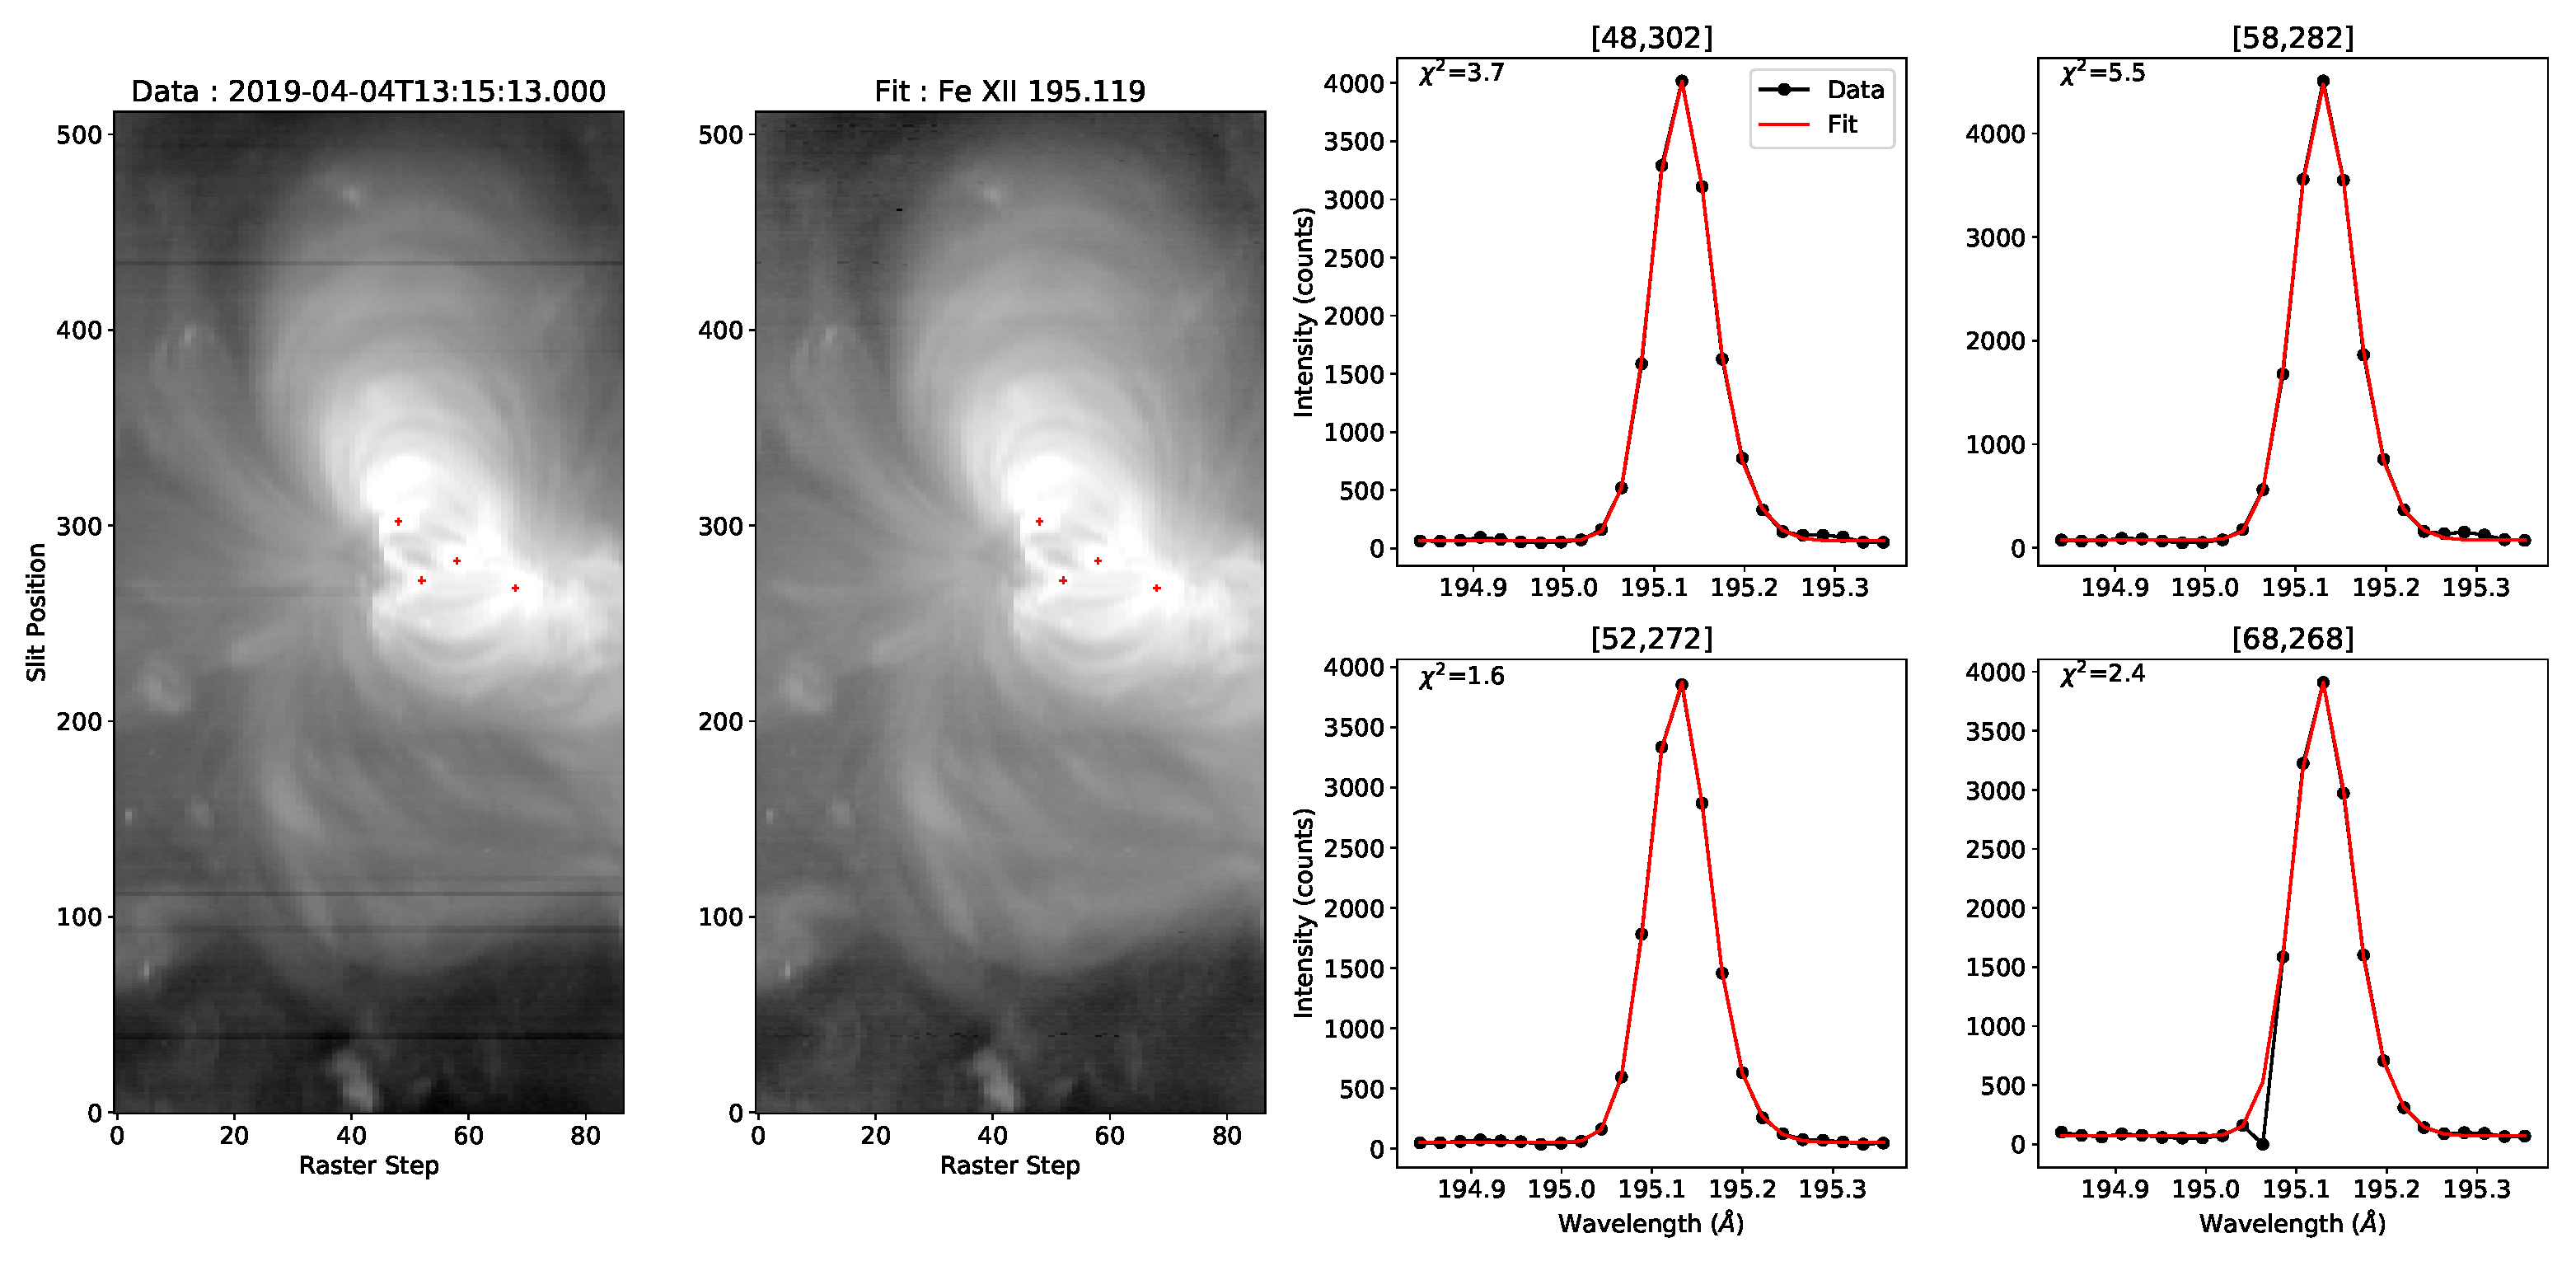
\includegraphics[clip,width=0.8\linewidth,bb=0 0 750 737]{figures/fit_example.pdf}}
  \centerline{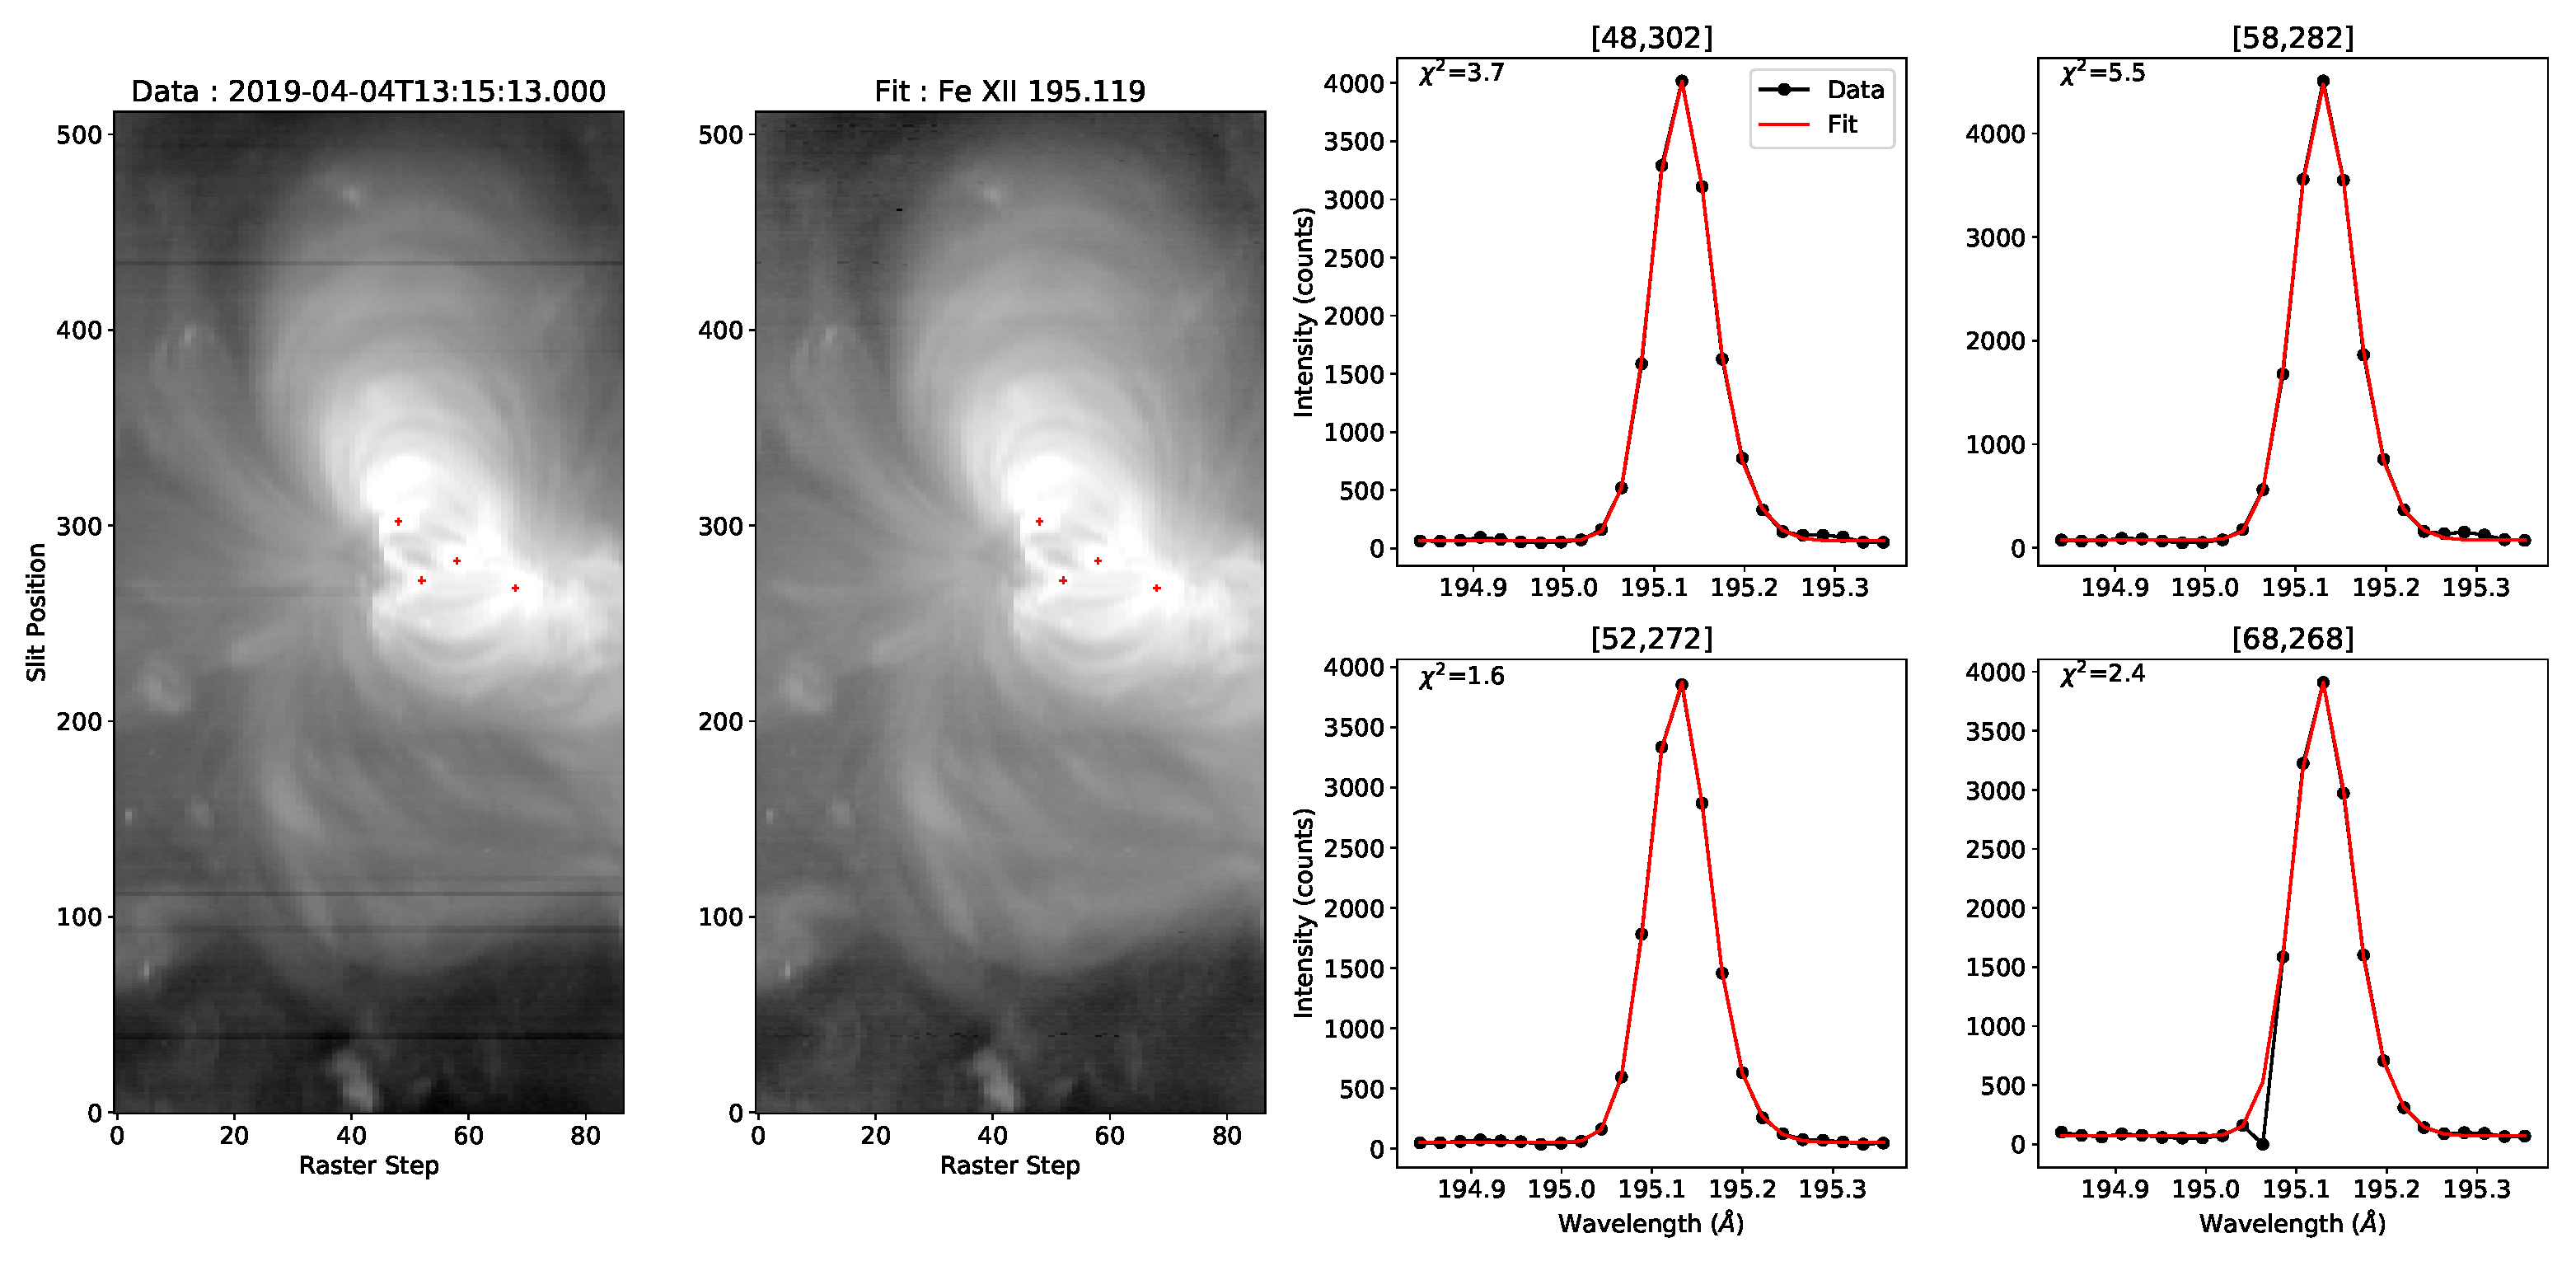
\includegraphics[clip,width=0.8\linewidth,bb=750 0 1500 737]{figures/fit_example.pdf}}  
  \caption{Example line profile fits. The top two panels show the raster formed by summing over the
    profile (left) and fitting each profile (right). The bottom panels show fits to four
    \ion{Fe}{12} 195.119\,\AA\ line profiles.}
  \label{fig:fit_example}
\end{figure}

As a final note about the fitting routines, there's also a parallelized version for fitting the raster that uses the Python Multiprocessing module \sidenote{This uses a pool of processes and parallelizes over the rasters so that each sub-process gets a raster position.}. When using the parallel version, an extra argument can be passed to the function to specify the number of processes to use (default=4) as in the below example. You can also check out the example in \verb+eis_fit_example_parallel.py+.

\begin{lstlisting}
fit = eis_fit_raster_parallel(wave, ints, errs, template, parinfo, ncpu=8)
\end{lstlisting}
